\subsection{Mel Frequency Cepstral Coefficients}
Ένα από τα χαρακτηριστικά που εξάγαμε από τα σήματα καρδιακών ήχων που είχαμε
στη διάθεση μας ώστε να εκπαιδεύσουμε το νευρωνικό δίκτυο είναι τα Mel Frequency
Cepstral Coefficients. Ο υπολογισμός τους έγινε στα ήδη προεπεργασμένα δεδομένα
και συγκεκριμένα στο κάθε ένα σήμα που δημιουργήθηκε από την έξοδο των
παραθύρων.Το συνόλο των συντελεστών που παρήγαγε αυτή η διαδικασία είναι 13 από
τους οποίους οι 12 αναπαριστούν την περισσότερη πληροφορία της φασματικής
περιβάλλουσας και ο 13\textsuperscript{ος} αναπαριστά τη συνολική ενέργεια του
σήματος. Δεν επιλέχθηκαν περισσότεροι από 13 συντελεστές καθώς η αύξηση του
αριθμού τους πάνω από αυτό το όριο έχει ως αποτέλεσμα την ταχεία μεταβολή των
συντελεστών γεγονός που δυσχαιρένει την εκπαίδευση του νευρωνικού δικτύου. Ο
κύριος λόγος που επιλέχθηκαν τα mfcc's είναι ότι αποτελούν την καλύτερη
προσέγγιση της λειτουργίας του κοχλία του ανθρώπινου αυτιού που είναι
επιλεκτικός στις συχνότητες και στο πως αντιδρά σε αυτές. Επιγραμματικά η
διαδικασία για τον υπολογισμό των mfcc είναι

\begin{itemize}
	\item Εφαρμογή παραθύρων στο σήμα
	\item Υπολογισμός του φάσματος ενέργειας
	\item Εφαρμογή του φίλτρου Mel και άθροισμα της ενέργειας του κάθε φίλτρου
	\item Λογαρίθμηση του αποτελέσματος του προηγούμενου βήματος
	\item Εφαρμογή μετασχηματισμού συνημιτόνων
\end{itemize}

\begin{figure}[H]
	\center
	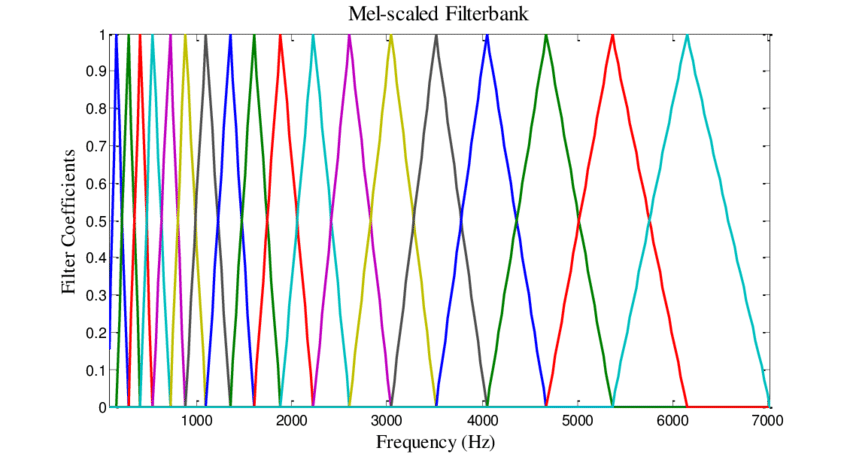
\includegraphics[width=0.8\textwidth]{images/MelFilter.png}
	\caption{Φίλτρο Mel}
	\label{melfilter}
\end{figure}


\subsection{Eξαγωγή στην Python}
Για τις ανάγκες υλοποίησης του νευρωνικού δικτύου ήταν απαραίτητη η εξαγωγή των
mfcc's από τα φωνοκαρδιογραφήματα  που είχαμε στη διάθεσή μας. Μετά την
προεπεξεργασία στην οποία υποβλήθηκαν όταν πλέον είχαμε τα δείγματα μας
χωρισμένα σε μικρότερα από επικαλυπτόμενα παράθυρα τότε σε κάθε ένα καινούριο
ηχητικό σήμα το οποίο είχε δημιουργηθεί εφαρμόστηκε η συνάρτηση mfcc της
βιβλιοθήκης \verb|python_speech_features| η έξοδος της οποίας, τα 13 mfcc's,
αποθηκεύτηκαν σε μορφή εικόνας που είναι και τα χαρακτηριστικά εκπαίδευσης  του
συνελικτικού νευρωνικού δικτύου.
